\documentclass[a4paper, twoside, 8pt]{extarticle}
\usepackage[
    left=1.2cm,
    right=1.2cm,
    top=2.25cm,
    bottom=1.25cm]{geometry}
\usepackage{multicol}

\usepackage{fancyhdr} % extensive control of page headers and footers
\makeatletter
\fancypagestyle{mypagestyle}
{\newpage \fancyfoot[C]{} \renewcommand{\footrulewidth}{0pt}}
\makeatother
\pagestyle{mypagestyle}
\headsep 5pt            

\usepackage[usenames,dvipsnames]{color} % colour control
\usepackage{xcolor} % driver-independent color extensions
\usepackage{amssymb} % provides an extended symbol collection

\usepackage{enumitem} % control layout of itemize, enumerate, description
\newenvironment{enumx} {
	\begin{enumerate}[leftmargin=*]
	\setlength{\topsep}{0pt}
	\setlength{\itemsep}{0pt}
	\setlength{\parskip}{0pt}
	\setlength{\parsep}{0pt}
	}
{\end{enumerate}}
\newenvironment{itemx} {
	\begin{itemize}[leftmargin=*,noitemsep,topsep=0pt]
	%\setlength{\itemsep}{0pt}
	%\setlength{\parskip}{0pt}
	%$\setlength{\parsep}{0pt}
	}
{\end{itemize}}

\usepackage{parskip} % layout with zero \parindent, non-zero \parskip
\usepackage{titlesec} % selects alternative section titles
\titlespacing\section{0pt}{6pt plus 4pt minus 2pt}{0pt plus 2pt minus 2pt}
\titlespacing\subsection{0pt}{6pt plus 4pt minus 2pt}{0pt plus 2pt minus 2pt}
\titlespacing\subsubsection{0pt}{6pt plus 4pt minus 2pt}{0pt plus 2pt minus 2pt}

\usepackage{lastpage} % reference last page
\usepackage{Alegreya}
\usepackage{hyperref}
\usepackage{minted}
\usepackage{tikz}

\newcommand{\manualbreak}{\vspace*{\fill}\columnbreak}
 
\usepackage[utf8]{inputenc}
\usepackage[T1]{fontenc}

\begin{document}
\renewcommand{\footrulewidth}{0.4pt}
\fancyhead[LE,LO]{TikZ/PGF -- cheat sheet (page \thepage/\pageref{LastPage})}
\fancyhead[RE,RO]{author: Remigiusz Suwalski, date: \today}
\fancyfoot[RF]{source: ?}
%\fancyfoot[LF]{}

\begin{multicols*}{2}
PGF (Portable Graphics Format) is an internal engine, 
whereas TikZ (TikZ ist kein Zeichenprogramm) serves as a frontend.

\section*{Usage}
\begin{minted}{tex}
% ...
\usepackage{tikz}

\begin{document}
\begin{tikzpicture}
% larger picture code here
\end{tikzpicture}
% ...
\end{minted}

\section*{Basic shapes}
\begin{minted}{tex}
\draw (10pt, 20pt) .. controls (30pt, 40pt) and (30pt, 20pt) 
   .. (10pt, 40pt);
\draw (40pt, 20pt) -- (60pt, 20pt) -- (50pt, 40pt) -- cycle; 
\draw (80pt, 30pt) circle (10pt);
\draw (105pt, 30pt) ellipse (5pt and 10pt);
\draw [->] (120pt, 20pt) -- (140pt, 40pt);
\end{minted}

\begin{center}
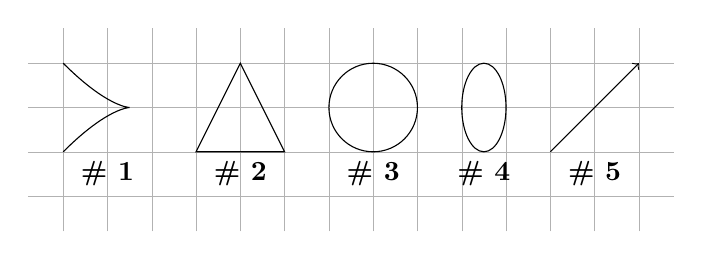
\begin{tikzpicture}[scale=1.6]
\draw[step=10 pt,black!30!white,ultra thin] (2 pt, 2 pt) grid (148 pt, 48 pt);
% grid
\draw (10pt, 20pt) .. controls (30pt, 40pt) and (30pt, 20pt) .. (10 pt, 40pt);
\node [below] at (20 pt, 20pt) {\textbf{\# 1}};
\draw (40pt, 20pt) -- (60pt, 20pt) -- (50pt, 40pt) -- cycle; 
\node [below] at (50 pt, 20pt) {\textbf{\# 2}};
\draw (80pt, 30pt) circle (10pt);
\node [below] at (80 pt, 20pt) {\textbf{\# 3}};
\draw (105pt, 30pt) ellipse (5pt and 10pt);
\node [below] at (105 pt, 20pt) {\textbf{\# 4}};
\draw [->] (120pt, 20pt) -- (140pt, 40pt);
\node [below] at (130pt, 20pt) {\textbf{\# 5}};
\end{tikzpicture}
\end{center}

\subsection*{Thickness}
\begin{minted}{tex}
\draw [ultra thick] (20pt, 20pt)  -- (20pt, 40pt);
\draw [very thick]  (40pt, 20pt)  -- (40pt, 40pt);
\draw [thick]       (60pt, 20pt)  -- (60pt, 40pt);
\draw [semithick]   (80pt, 20pt)  -- (80pt, 40pt);
\draw [thin]        (100pt, 20pt) -- (100pt, 40pt);
\draw [very thin]   (120pt, 20pt) -- (120pt, 40pt);
\draw [ultra thin]  (140pt, 20pt) -- (140pt, 40pt);
\end{minted}

\begin{center}
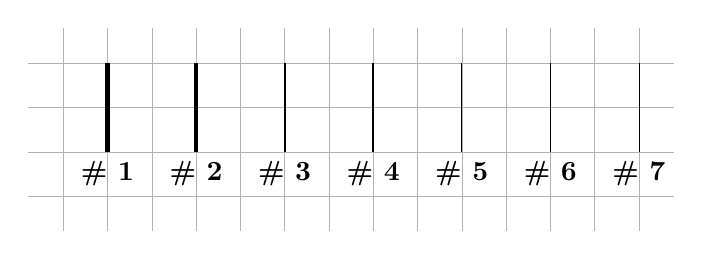
\begin{tikzpicture}[scale=1.6]
\draw[step=10 pt,black!30!white,ultra thin] (2 pt, 2 pt) grid (148 pt, 48 pt);
% grid
\draw [ultra thick] (20pt, 20pt)  -- (20pt, 40pt);
\node [below] at (20 pt, 20pt) {\textbf{\# 1}};
\draw [very thick]  (40pt, 20pt)  -- (40pt, 40pt);
\node [below] at (40 pt, 20pt) {\textbf{\# 2}};
\draw [thick]       (60pt, 20pt)  -- (60pt, 40pt);
\node [below] at (60 pt, 20pt) {\textbf{\# 3}};
\draw [semithick]   (80pt, 20pt)  -- (80pt, 40pt);
\node [below] at (80 pt, 20pt) {\textbf{\# 4}};
\draw [thin]   (100pt, 20pt) -- (100pt, 40pt);
\node [below] at (100 pt, 20pt) {\textbf{\# 5}};
\draw [very thin]        (120pt, 20pt) -- (120pt, 40pt);
\node [below] at (120 pt, 20pt) {\textbf{\# 6}};
\draw [ultra thin]  (140pt, 20pt) -- (140pt, 40pt);
\node [below] at (140 pt, 20pt) {\textbf{\# 7}};
\end{tikzpicture}
\end{center}

\subsection*{Dots and dashes}
All lines drawn below are ultra thick.

\begin{minted}{tex}
\draw [ultra thick, densely dotted];
\draw [ultra thick, dotted];
\draw [ultra thick, loosely dotted];
\draw [ultra thick, densely dashed];
\draw [ultra thick, dashed];
\draw [ultra thick, loosely dashed];
\draw [ultra thick, dashdotted];
\end{minted}

\begin{center}
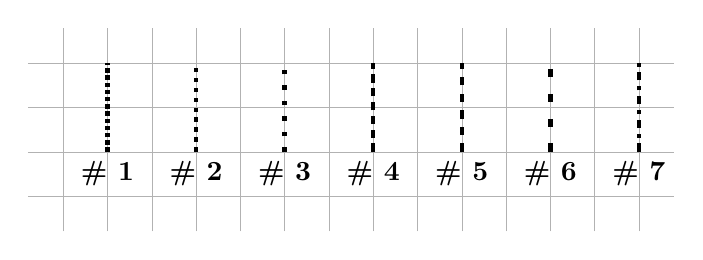
\begin{tikzpicture}[scale=1.6]
\draw[step=10 pt,black!30!white,ultra thin] (2 pt, 2 pt) grid (148 pt, 48 pt);
% grid
\draw [ultra thick, densely dotted] (20pt, 20pt) -- (20pt, 40pt);
\node [below] at (20 pt, 20pt) {\textbf{\# 1}};
\draw [ultra thick, dotted] (40pt, 20pt) -- (40pt, 40pt);
\node [below] at (40 pt, 20pt) {\textbf{\# 2}};
\draw [ultra thick, loosely dotted] (60pt, 20pt) -- (60pt, 40pt);
\node [below] at (60 pt, 20pt) {\textbf{\# 3}};
\draw [ultra thick, densely dashed] (80pt, 20pt) -- (80pt, 40pt);
\node [below] at (80 pt, 20pt) {\textbf{\# 4}};
\draw [ultra thick, dashed] (100pt, 20pt) -- (100pt, 40pt);
\node [below] at (100 pt, 20pt) {\textbf{\# 5}};
\draw [ultra thick, loosely dashed] (120pt, 20pt) -- (120pt, 40pt);
\node [below] at (120 pt, 20pt) {\textbf{\# 6}};
\draw [ultra thick, dashdotted] (140pt, 20pt) -- (140pt, 40pt);
\node [below] at (140 pt, 20pt) {\textbf{\# 7}}; 
\end{tikzpicture}
\end{center}

\vfill\null

\subsection*{Available colours}
\begin{multicols*}{3}
$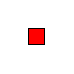
\begin{tikzpicture}[scale=0.5, baseline=-0.65ex]
\filldraw[fill=red, draw=black] (-6pt, -6pt) rectangle (6pt, 6pt);
\end{tikzpicture}$ \, red

$
\begin{tikzpicture}[scale=0.5, baseline=-0.65ex]
\filldraw[fill=green, draw=black] (-6pt, -6pt) rectangle (6pt, 6pt);
\end{tikzpicture}$ \, green

$
\begin{tikzpicture}[scale=0.5, baseline=-0.65ex]
\filldraw[fill=blue, draw=black] (-6pt, -6pt) rectangle (6pt, 6pt);
\end{tikzpicture}$ \, blue

$
\begin{tikzpicture}[scale=0.5, baseline=-0.65ex]
\filldraw[fill=cyan, draw=black] (-6pt, -6pt) rectangle (6pt, 6pt);
\end{tikzpicture}$ \, cyan

$
\begin{tikzpicture}[scale=0.5, baseline=-0.65ex]
\filldraw[fill=magenta, draw=black] (-6pt, -6pt) rectangle (6pt, 6pt);
\end{tikzpicture}$ \, magenta

$
\begin{tikzpicture}[scale=0.5, baseline=-0.65ex]
\filldraw[fill=yellow, draw=black] (-6pt, -6pt) rectangle (6pt, 6pt);
\end{tikzpicture}$ \, yellow

$
\begin{tikzpicture}[scale=0.5, baseline=-0.65ex]
\filldraw[fill=black, draw=black] (-6pt, -6pt) rectangle (6pt, 6pt);
\end{tikzpicture}$ \, black

$
\begin{tikzpicture}[scale=0.5, baseline=-0.65ex]
\filldraw[fill=gray, draw=black] (-6pt, -6pt) rectangle (6pt, 6pt);
\end{tikzpicture}$ \, gray

$
\begin{tikzpicture}[scale=0.5, baseline=-0.65ex]
\filldraw[fill=darkgray, draw=black] (-6pt, -6pt) rectangle (6pt, 6pt);
\end{tikzpicture}$ \, darkgray

$
\begin{tikzpicture}[scale=0.5, baseline=-0.65ex]
\filldraw[fill=lightgray, draw=black] (-6pt, -6pt) rectangle (6pt, 6pt);
\end{tikzpicture}$ \, lightgray

$
\begin{tikzpicture}[scale=0.5, baseline=-0.65ex]
\filldraw[fill=brown, draw=black] (-6pt, -6pt) rectangle (6pt, 6pt);
\end{tikzpicture}$ \, brown

$
\begin{tikzpicture}[scale=0.5, baseline=-0.65ex]
\filldraw[fill=lime, draw=black] (-6pt, -6pt) rectangle (6pt, 6pt);
\end{tikzpicture}$ \, lime

$
\begin{tikzpicture}[scale=0.5, baseline=-0.65ex]
\filldraw[fill=olive, draw=black] (-6pt, -6pt) rectangle (6pt, 6pt);
\end{tikzpicture}$ \, olive

$
\begin{tikzpicture}[scale=0.5, baseline=-0.65ex]
\filldraw[fill=orange, draw=black] (-6pt, -6pt) rectangle (6pt, 6pt);
\end{tikzpicture}$ \, orange

$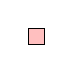
\begin{tikzpicture}[scale=0.5, baseline=-0.65ex]
\filldraw[fill=pink, draw=black] (-6pt, -6pt) rectangle (6pt, 6pt);
\end{tikzpicture}$ \, pink

$
\begin{tikzpicture}[scale=0.5, baseline=-0.65ex]
\filldraw[fill=purple, draw=black] (-6pt, -6pt) rectangle (6pt, 6pt);
\end{tikzpicture}$ \, purple

$
\begin{tikzpicture}[scale=0.5, baseline=-0.65ex]
\filldraw[fill=teal, draw=black] (-6pt, -6pt) rectangle (6pt, 6pt);
\end{tikzpicture}$ \, teal

$
\begin{tikzpicture}[scale=0.5, baseline=-0.65ex]
\filldraw[fill=violet, draw=black] (-6pt, -6pt) rectangle (6pt, 6pt);
\end{tikzpicture}$ \, violet

$\begin{tikzpicture}[scale=0.5, baseline=-0.65ex]
\filldraw[fill=white, draw=black] (-6pt, -6pt) rectangle (6pt, 6pt);
\end{tikzpicture}$~\, white
\end{multicols*}
\end{multicols*}
\end{document}
